\documentclass[10pt,a4paper,twocolumn]{article}
\usepackage[left=13.5mm,right=13.5mm,top=17mm,bottom=17mm,columnsep=5mm]{geometry}
\usepackage{nature_reading}
\brokenpenalty=10000
\begin{document}
\twocolumn[{\noindent{\sffamily\bfseries\fontsize{23}{26}\selectfont
Question-conditioned writing in image space\par}
\vspace{7pt}\noindent Imagized Language Model Project\par
\vspace{9pt}\noindent\textbf{Methods companion, 5 November 2026.}
Question-dependent writing is a requirement for an independent image-language
model. This note specifies a registered paired training objective and its
completed implementation preflight. Autonomous-language performance is not
established by these implementation checks.
\par\vspace{9pt}
\centering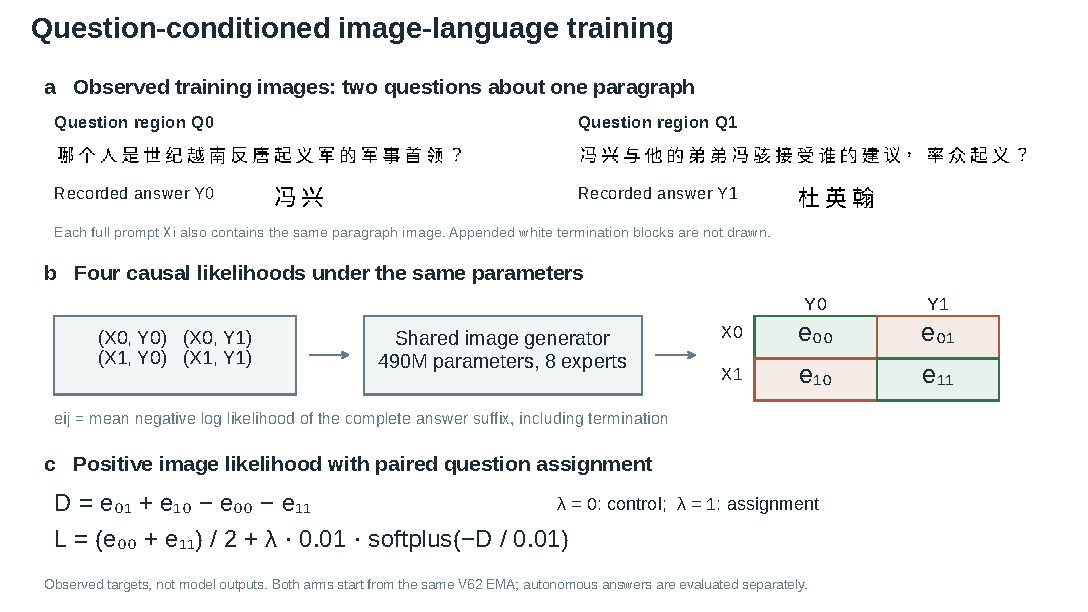
\includegraphics[width=.99\textwidth]{question_assignment_method.pdf}
\captionsetup{hypcap=false}
\captionof{figure}{\textbf{Paired image-language training.}
\textbf{a,} Question regions and observed answer images from the first admitted
training pair. Each full prompt also contains the shared paragraph, omitted
from display. Targets retain native padding; appended white termination blocks
are not drawn. These are training data, not model-generated answers.
\textbf{b,} One image generator scores all four causal prompt--answer streams.
Diagonal cells are own-question targets; off-diagonal cells are swapped targets.
The $e_{ij}$ labels are symbolic energies, not numerical measurements.
\textbf{c,} Positive image likelihood is supplemented by an assignment loss.
The two arms share initialization, architecture, sampled pairs and update
budget, differing in $\lambda$. Actual free answers and question controls
are evaluated separately.}\label{fig:method}
\vspace{9pt}}]

\section*{Physical observations and targets}
The source is a short-answer Chinese reading subset of CMRC~2018\cite{cmrc}:
3,211 training questions and 1,321 reused development questions, with original
article overlap removed. Training pairs share a paragraph and have disjoint
retained answer strings and canonical reference-image sequences. Admission
retains 3,793 pairs across 939 paragraphs and 3,016 distinct questions. Two
pairs sharing an accepted answer string are excluded. Paragraphs, then valid
pairs within them, are sampled uniformly.

Each $X_i$ is the complete observed prompt image. Each $Y_j$ is a padded
answer-image suffix followed by two white termination blocks. The actor reads
binary $32\!\times\!64$ physical image blocks; it receives no character IDs,
answer location, glyph inventory or external language-model response. Host
rendering of source text is data preparation, outside the actor boundary.

\section*{Conditional image probability}
The contextual backbone is externally pretrained MIXAR-477M\cite{mixar},
adapted with eight conditional bitmap experts. All~489,998,208 actor parameters
participate in training. For~an answer block with 2,048 white/ink bits (one
denotes white),
\begin{equation}
p_\theta(y_t\mid h_t)=\sum_{k=1}^{8}\pi_k(h_t)
\prod_{u=1}^{2048}\operatorname{Bern}
\bigl(y_{tu};\sigma(a_{ku}(h_t))\bigr).
\end{equation}
The gate is normalized, and every expert defines a normalized bitmap law.
Thus the mixture is normalized. Each expert is a context-dependent neural
function, with no fixed character identity. The causal state $h_t$ sees the
prompt and preceding answer blocks. Future target blocks cannot enter an
earlier prediction. The suffix probability is the product of these block
conditionals.

\section*{Paired objective}
Let $n_j$ be the number of scored pixels in the complete suffix $Y_j$,
including termination. Define
\begin{align}
e_{ij}&=-\frac{1}{n_j}\log p_\theta(Y_j\mid X_i),\\
D&=e_{01}+e_{10}-e_{00}-e_{11},\\
L&=\frac{e_{00}+e_{11}}{2}
+\lambda\tau\operatorname{softplus}(-D/\tau),\quad\tau=0.01.
\end{align}
The control uses $\lambda=0$; assignment training uses $\lambda=1$. Both arms
compute the same four likelihood graphs. Teacher forcing supplies observed
answer pixels only after their causal predecessors.

Adding arbitrary row and column offsets $a_i+b_j$ to $e_{ij}$ leaves $D$
unchanged, because each offset occurs once with each sign. The derivative of
the assignment term with respect to $D$ is $-\sigma(-D/\tau)$. This elementary
identity describes a training signal, not a theorem of semantic learning.
For equal $n_0=n_1=n$, $D$ equals $1/n$ times the log ratio of correct to swapped
joint assignments. With unequal lengths, it is a length-normalized interaction
energy and must not be called that single joint log odds or a mutual-information
estimate. Feature interactions such as question/answer width can still support
ranking without useful writing.

\balance
\section*{Registered comparison}
Both arms start from the same learned V62 eight-expert EMA. Each makes 2,000
updates, accumulating four pairs per update: eight positive and eight swapped
streams. AdamW uses learning rate $2\!\times\!10^{-5}$, betas $(0.9,0.95)$,
weight decay $0.01$, 100-step warmup, cosine decay to one tenth, norm clipping
at one and EMA coefficient $0.99$. Parameters, optimizer and EMA use FP32;
forward/backward use BF16 autocast, deterministic eager attention and
nonreentrant activation checkpointing. The final EMA is fixed in advance;
development scores do not select checkpoints or seeds. Arms run sequentially
on physical GPU~0, with a 20-GiB allocated-memory and eight-hour limit per arm.
External foundation pretraining is separate from local adaptation cost.

\section*{Completed implementation preflight}
All 26 implementation checks pass using training data only. A full optimizer
and EMA update on the longest admitted joined stream, 250 image blocks with
all four graphs retained, peaks at 9.197~GiB. Four-update checks peak at
9.235~GiB for either arm. Four uninterrupted updates exactly match two plus
resumed two in model, EMA, optimizer, Python/NumPy/Torch CPU/CUDA RNG, pair RNG
and the complete sampled-pair journal, independently for each arm.

All parameter gradients are finite. Assignment-only gradients are nonzero
through the physical input projection, first/last contextual layers, bitmap
projection and mixture gate. Physical four-stream assembly matches the source
prefix/suffix tensors. Changing future answer pixels gives zero earlier-output
change. Strict-FP32 cached/prefill maximum logit difference is
$6.485\!\times\!10^{-5}$, within the registered $2\!\times\!10^{-4}$ tolerance.
These checks establish implementation feasibility; they do not establish
language accuracy or efficiency at matched capability.

\section*{Inference and independent assessment}
The deployed actor generates physical bitmap candidates, scores them under
the complete mixture and feeds selected pixels back into its visual context.
Searching expert threshold modes is approximate MAP, not a guaranteed global
mode. An all-white block stops writing. No malformed image is repaired,
snapped to a character bank or replaced by a font glyph.

The locked audit follows both completed training arms and independent offline
deployment replay. It retains 256 primary questions, all 393 shared-paragraph
pairs and all 1,321 development likelihood cases, with normal and blank-question
controls. The bounded reading requirements include at least 10\% exact primary
answers, 25\% strict-raster F1, 2\% both-correct pairs, fewer than 20\% capped
outputs and a positive lower bound of the 95\% article-bootstrap interval for
the question effect.
The assignment intervention additionally requires a positive lower bound for
its raster-F1 gain over control. Reference-answer energy ranking is diagnostic
and cannot replace autonomous answers. No outcome from that audit is reported
in this methods companion.

Canonical font shift, reused development, one training seed, externally
pretrained weights and short extractive answers limit interpretation. Useful
general Chinese/English instruction following, books and historical writing
remain distinct requirements. Code, fixed protocol, preflight and image-source
hashes accompany this note; the complete primary record remains in the
repository.

\begin{thebibliography}{2}
\bibitem{cmrc} Cui, Y. et al. A Span-Extraction Dataset for Chinese Machine
Reading Comprehension. \emph{Proceedings of EMNLP-IJCNLP}, 5883--5889 (2019).
\url{https://aclanthology.org/D19-1600/}.
\bibitem{mixar} Hu, C., Tai, Y., Vergari, A., Keller, F. \& Suglia, A. MIXAR:
Scaling Autoregressive Pixel-based Language Models to Multiple Languages and
Scripts. \emph{arXiv} 2604.11575v2 (2026).
\url{https://arxiv.org/abs/2604.11575v2}.
\end{thebibliography}
\end{document}
